%!TEX ROOT=formularioMatematica.tex

\section{Geometria analitica}\label{sec:geomanal}
La geometria analitica � la geometria che si occupa di lavorare nel piano cartesiano ($xOy$).\\
Per gli esercizi si vada \hyperref[ex:geomanal]{qui}.

\subsection{Generale}
Le formule qui riportate sono generali a tutto l'ambito della geometria analitica e non si riferiscono
ad una figura particolare.\\
Di seguito viene rappresentato il tipico piano cartesiano con i suoi quattro quadranti.
\begin{center}
	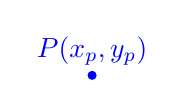
\begin{tikzpicture}
		\tkzInit[xmin=-3,ymin=-3,xmax=3,ymax=3]
		\tkzGrid
		\tkzAxeXY
		\filldraw[blue] (-1,2) circle (0.05)
			node[above]{$P(x_p, y_p)$};
	\end{tikzpicture}
\end{center}
D'ora in poi, si dar� per scontata la convenzione di nominare le coordinate di un punto in base al nome
del punto stesso. Ad esempio $P(x_P, y_P)$. Si noti anche che � possibile definire un punto attraverso
un vettore bidimensionale. Ovvero
\begin{equation*}
P(x_P,y_P) = \begin{bmatrix}
x_P\\y_P
\end{bmatrix}
\end{equation*}

\subsubsection{Distanza tra due punti}
\begin{equation*}
\overline{AB} = \sqrt{(x_B-x_A)^2+(y_B-y_A)^2}
\end{equation*}

\subsubsection{Punto medio}
\begin{equation*}
M\left(\frac{x_A-x_B}{2}, \frac{y_A-y_B}{2}\right)
\end{equation*}

\subsubsection{Punto su un segmento in un rapporto $\frac{m}{n}$}
Siano $m$ e $n$ due rapporti a cui sta un punto rispetto al segmento. Ovvero il punto $P(x_P, y_P)$
divide il segmento in $n$ parti sulla proiezione della $x$, in $m$ parti su quella di $y$.
\begin{equation*}
P\left(\frac{nx_A+mx_B}{m+n},\frac{ny_A+my_B}{m+n}\right)
\end{equation*}

\subsubsection{Baricentro di un triangolo}
\begin{equation*}
G\left(\frac{x_A+x_B+x_C}{3},\frac{y_A+y_B+y_C}{3}\right)
\end{equation*}

\subsubsection{Area di un poligono qualsiasi}
\begin{equation*}
\mathscr{A}(P) = \frac{1}{2}\left\lvert 
\begin{matrix}[1]
x_1 & y_1 & 1\\
x_2 & y_2 & 1\\
x_3 & y_3 & 1\\
\vdots & \vdots & 1
\end{matrix}\right\rvert
\end{equation*}
usando la regola di Sarrus. Questa formula � anche chiamata la formula di Gauss per le aree di 
poligoni.\\
Il modo di calcolare il determinante (o valore) della matrice � il seguente (in definitiva andare
in diagonale dall'alto per ogni elemento della prima colonna moltiplicando gli elementi e quando si
cambia colonna si sommi. Andare poi dal basso sottraendo).\\
Il determinante della matrice
\begin{equation*}
\begin{bmatrix}[1]
a_{11} & a_{12} & a_{13}\\
a_{21} & a_{22} & a_{23}\\
a_{31} & a_{32} & a_{33}
\end{bmatrix}
\end{equation*}
� dato dalla risoluzione come descritto di questo
\begin{center}
	\begin{tikzpicture}[baseline=(A.center), scale=0.5]
	\tikzset{node style ge/.style={circle}}
	\tikzset{bar/.style = {opacity=.3,line width=4 mm,line cap=round,color=#1}}
	\tikzset{plus/.style = {above left,,opacity=1,circle,fill=#1!50}}
	\tikzset{minus/.style = {below left,,opacity=1,circle,fill=#1!50}}
	
	\matrix (A) [matrix of math nodes, nodes = {node style ge},,column sep=0 mm] 
	{ a_{11} & a_{12} & a_{13}\\
		a_{21} & a_{22} & a_{23}\\
		a_{31} & a_{32} & a_{33}\\
		a_{11} & a_{12} & a_{13}\\
		a_{21} & a_{22} & a_{13}\\
	};
	
	\draw [bar=blue] (A-1-1.north west) node[plus=blue] {$+$} to (A-3-3.south east);
	\draw [bar=blue] (A-2-1.north west) node[plus=blue] {$+$} to (A-4-3.south east);
	\draw [bar=blue] (A-3-1.north west) node[plus=blue] {$+$} to (A-5-3.south east);
	\draw [bar=red]  (A-3-1.south west) node[minus=red] {$-$} to (A-1-3.north east);
	\draw [bar=red]  (A-4-1.south west) node[minus=red] {$-$} to (A-2-3.north east);
	\draw [bar=red]  (A-5-1.south west) node[minus=red] {$-$} to (A-3-3.north east);
	\end{tikzpicture}
\end{center}
che contiene una ripetizione di tutte le righe tranne l'ultima. Volendo si pu� "saltare" all'inizio
per evitare di scrivere la ripetizione per� in questo modo si � sicuri di non sbagliare.

\subsection{Rette}\label{subsec:geomanal:retta}
\begin{center}
	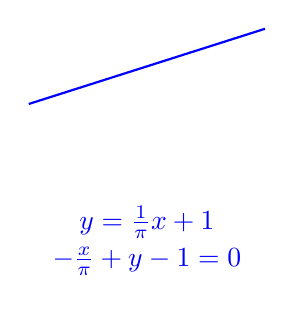
\begin{tikzpicture}
		\tkzInit[xmin=0,ymin=0,xmax=3,ymax=3]
		\tkzGrid
		\tkzAxeXY
		\draw[blue, thick, domain=0:3] plot(\x,1/pi*\x+1);
		\node[blue] (l) at (1.5,-0.5){$y = \frac{1}{\pi}x+1$};
		\node[blue] (l1) at (1.5,-1){$-\frac{x}{\pi} + y - 1 = 0$};
	\end{tikzpicture}
\end{center}
Le rette sono definite da un'equazione che ha due forme equivalenti:
\begin{equation}\label{eq:retta1}
y = mx + q\\
\end{equation}
\begin{equation}\label{eq:retta2}
ax + by + c = 0
\end{equation}
La forma \eqref{eq:retta1} � chiamata \emph{esplicita}, la forma \eqref{eq:retta2} � chiamata 
\emph{implicita}. Da queste due forme possiamo evincere che
\begin{equation*}
m = -\frac{a}{b} \qquad q = -\frac{c}{b}
\end{equation*}
% Reset the counter
\setcounter{equation}{0}

\subsubsection{Retta passante per due punti $P_1(x_1,y_1)$ e $P_2(x_2,y_2)$}
\begin{equation*}
\frac{y-y_1}{y_2-y_1}=\frac{x-x_1}{x_2-x_1} \qquad x_1\neq x_2 \land y_1\neq y_2
\end{equation*}

\subsubsection{Condizione di parallelismo}
Perch� due rette siano parallele, \textbf{il loro coefficiente angolare deve essere uguale}, ovvero
\begin{equation*}
r_1 \| r_2 \iff m_1=m_2
\end{equation*}

\subsubsection{Condizione di perpendicolarit�}
Perch� due rette siano perpendicolari, \textbf{il prodotto dei coefficienti angolari deve essere $-1$},
ovvero
\begin{equation*}
r_1 \perp r_2 \iff m_1m_2 = -1
\end{equation*}

\subsubsection{Retta parallela ad una data e passante per un punto $P(x_P,y_P)$}
\begin{equation*}
y-y_P = m(x-x_P)
\end{equation*}

\subsubsection{Retta perpendicolare ad una data e passante per un punto $P(x_P,y_P)$}
\begin{equation*}
y - y_P = -\frac{1}{m} (x - x_P)
\end{equation*}

\subsubsection{Distanza $d$ tra un punto $P(x_P,y_P)$ e una retta}
\begin{equation*}
d = \frac{\abs{ax_P + by_P +c}}{\sqrt{a^2+b^2}}
\end{equation*}

\subsubsection{Coefficiente angolare $m$ di una retta passante per due punti $P_1(x_1,y_1)$ e 
$P_2(x_2,y_2)$}
\begin{equation*}
m=\frac{y_2-y_1}{x_2-x_1}
\end{equation*}

\subsection{Fasci di Rette}\label{subsec:geomanal:fasciorette}
Un fascio di rette � una combinazione lineare di tutte le rette generabili modificando un solo 
parametro di una quantit� costante.

\subsubsection{Fascio di rette a due parametri}
Sceglti appropriati $\alpha$ e $\beta$ si possono generare tutte le rette possibili utilizzando questa
forma
\begin{equation*}
\alpha(ax + by + c) + \beta(a_1x + b_1y + c_1) = 0
\end{equation*}
\begin{equation*}
(\alpha a + \beta a_1)x + (\alpha b + \beta b_1)y + \alpha c + \beta c_1 = 0
\end{equation*}

\subsubsection{Fascio di rette ad un parametro}
Questa forma esclude una sola retta, per $k = 0$.
\begin{equation*}
ax + by + c + k(a_1x + b_1y + c_1) = 0
\end{equation*}
Si noti che $k = \frac{\beta}{\alpha}$

\subsubsection{$k$ avendo una retta del fascio, la retta esclusa e un punto su $a_1x + b_1y + c = 0$}
\begin{center}
	\begin{tikzpicture}
		\draw[teal, dashed] (0,-0.15) -- (3,-0.15)
			node[pos=0, above left]{Esclusa: $a_1x + b_1y + c = 0$};
		\draw[brown] (0,-3) -- (2,1)
			node[pos=0, below]{$r: ax + by + c = 0$};
		\draw[red] (2.5,-3) -- (1,1)
			node[pos = 0.5, left]{$k = ?$};
		\filldraw[blue] (2,-1.65) circle(0.05)
			node[right]{$Q(x_Q, y_Q)$};
	\end{tikzpicture}
\end{center}
\begin{equation*}
\mathcolor{red}{k} = -\frac{
	\mathcolor{brown}{a}\mathcolor{blue}{x_Q} + \mathcolor{brown}{b}\mathcolor{blue}{y_Q} +
	\mathcolor{brown}{c}
}{
	\mathcolor{teal}{a_1}\mathcolor{blue}{x_Q} + \mathcolor{teal}{b_1}\mathcolor{blue}{y_Q} +
	\mathcolor{teal}{c_1}
}
\end{equation*}

\subsubsection{Retta di un fascio con coefficiente angolare $m$ passante per un punto $P(x_P,y_P)$}
\begin{equation*}
y-y_P = m(x-x_P)
\end{equation*}

\subsection{Circonferenza}\label{subsec:geomana:circ}
La circonferenza � una conica i cui punti sono tutti equidistanti dal centro $C$.
\begin{center}
	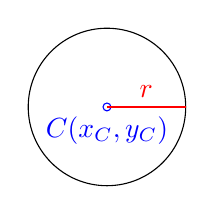
\begin{tikzpicture}
		\draw (0,0) circle (1);
		\draw[blue] (0,0) circle (0.05)
			node[below]{$C(x_C, y_C)$};
		\draw[red] (0,0) -- (1,0)
			node[pos=0.5,above]{$r$};
	\end{tikzpicture}
\end{center}

Anche le equazioni delle circonferenze hanno 2 forme
\begin{equation*}
\mathscr{C}:\,(x-\mathcolor{blue}{x_C})^2 + (y-\mathcolor{blue}{y_C})^2 = \mathcolor{red}{r}^2
\end{equation*}
\begin{equation*}
\mathscr{C}:\,x^2+y^2+ax+by+c =0
\end{equation*}
Da queste due formule derivano le coordinate del centro
\begin{equation*}
C\left(-\frac{a}{2},-\frac{b}{2}\right)
\end{equation*}
e la misura del raggio
\begin{equation*}
\mathcolor{red}{r} = \sqrt{\mathcolor{blue}{x_C}^2+\mathcolor{blue}{y_C}^2-c} = 
\sqrt{\frac{a^2}{4}+\frac{b^2}{4}-c}
\end{equation*}

\subsubsection{Tangente in $P(x_P,y_P)$}
\begin{equation*}
x\cdot x_P+y\cdot y_P+a\frac{x+x_P}{2}+b\frac{y+y_P}{2}+c = 0
\end{equation*}

\subsubsection{Area del cerchio}
\begin{equation*}
\mathscr{A}(\mathscr{C}) = \pi\mathcolor{red}{r}^2
\end{equation*}

\subsubsection{Lunghezza della circonferenza}
\begin{equation*}
C = 2\pi\mathcolor{red}{r}
\end{equation*}

\subsubsection{Lunghezza dell'arco}
\begin{equation*}
l = \mathcolor{red}{r}\alpha
\end{equation*}
Si noti che $\alpha$ � in radianti.

\subsubsection{Area del settore}
\begin{equation*}
\mathscr{A}(\mathscr{S}) = \frac{1}{2}\mathcolor{red}{r}^2\alpha
\end{equation*}
Si noti che $\alpha$ � in radianti.

\subsection{Fasci di circonferenze}\label{subsec:geomanal:fasciocirc}
Un fascio di circonferenze � una combinazione lineare di utte le circonferenze generabili modificando
un parametro di una certa quantit� costante.

\subsubsection{Fascio di circonferenze ad un parametro}
Scelti appropriati $\alpha$ e $\beta$ si possono generare tute le circonferenze possibili utilizzando 
questa forma
\begin{equation*}
\alpha(x^2+y^2+a_1x+b_1y+c_1) + \beta(x^2+y^2+a_2x+b_2y+c_2) = 0
\end{equation*}
\begin{equation*}
(\alpha+\beta)x^2+(\alpha+\beta)y^2+(\alpha a_1+\beta a_2)x+(\alpha b_1+\beta b_2)y+
\alpha c_1+\beta c_2 = 0
\end{equation*}

\subsubsection{Fascio di circonferenze a due parametri}
Questa forma esclude una circonferenza per $k=0$.
\begin{equation*}
x^2+y^2+ax+by+c+k(x^2+y^2+a_1x+b_1y+c_1) = 0
\end{equation*}
Si noti che $k=\frac{\alpha}{\beta}$

\subsection{Parabola}\label{subsec:geomanal:parabola}
\begin{center}
	\begin{tikzpicture}
		\tkzInit[xmin=-2,ymin=-2,xmax=4,ymax=4]
		\tkzGrid
		\tkzAxeXY

		\draw[red,domain=-2:2] plot(\x, \x*\x);
		\draw[blue,domain=-2:2] plot(\x*\x,\x);
	\end{tikzpicture}
\end{center}
Una parabola pu� essere descritta con l'asse focale parallelo all'asse $x$ o all'asse $y$.
\begin{equation*}
\mathcolor{red}{\mathscr{P}}:\,y=ax^2+bx+c
\end{equation*}
\begin{equation*}
\mathcolor{blue}{\mathscr{P}}:\,x=ay^2+by+c
\end{equation*}
La direttrice di una parabola � quella che ne da l'inclinazione ed � perpendicolare all'asse di
simmetria.\\
Il vertice di una parabola � il punto pi� vicino alla direttrice.\\
Il fuoco � il punto la cui distanza da qualsiasi punto della parabola � pari a quella della proiezione
sulla direttrice del punto stesso.

\subsubsection{Elementi di una parabola con asse focale parallelo a $x$}
\begin{center}
	\begin{tabular}{c | c}
		\textbf{Vertice} & $\left(-\dfrac{b}{2a}, -\dfrac{\Delta}{4a}\right)$\\\hline
		\textbf{Fuoco} & $\left(-\dfrac{b}{2a},\dfrac{1-\Delta}{4a}\right)$\\\hline
		\textbf{Direttrice} & $y=-\dfrac{1+\Delta}{4a}$\\\hline
		\textbf{Asse di simmetria} & $x=-\dfrac{b}{2a}$\\\hline
		\textbf{Tangente in un punto} & $\dfrac{y+y_0}{2}=axx_0+b\dfrac{x+x_0}{2}+c$
	\end{tabular}
\end{center}

\subsubsection{Elementi di una parabola con asse focale parallelo a $y$}
\begin{center}
	\begin{tabular}{c | c}
		\textbf{Vertice} & $\left(-\dfrac{\Delta}{4a},-\dfrac{b}{2a}\right)$\\\hline
		\textbf{Fuoco} & $\left(\dfrac{1-\Delta}{4a},-\dfrac{b}{2a}\right)$\\\hline
		\textbf{Direttrice} & $x=-\dfrac{1+\Delta}{4a}$\\\hline
		\textbf{Asse di simmetria} & $y=-\dfrac{b}{2a}$\\\hline
		\textbf{Tangente in un punto} & $\dfrac{x+x_0}{2}=ayy_0+b\dfrac{y+y	_0}{2}+c$
	\end{tabular}
\end{center}

\subsubsection{Parabole di vertice $V(x_V,y_V)$}
\begin{equation*}
y-y_V=a(x-x_V)^2
\end{equation*}

\subsubsection{Area di un segmento parabolico}
\begin{center}
	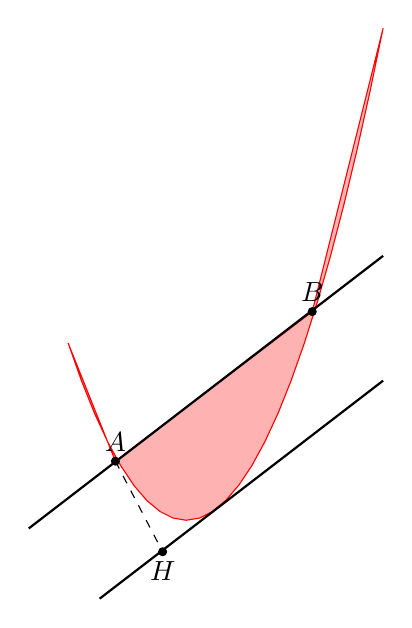
\begin{tikzpicture}
		\tkzInit[xmin=-1.5,ymin=-1,xmax=2.5,ymax=6]
		\tkzGrid
		\tkzAxeXY
		
		\filldraw[red, domain=-1.5:2.5, fill opacity=0.3](-0.9,0.75)--plot(\x, \x*\x)--(1.6,2.65)--
		cycle;
		\draw[thick, domain=-2:2.5] plot(\x, {\x/1.3+3.3/2.3});
		\draw[thick, domain=-1.1:2.5] plot(\x, {\x/1.3-0.15});
		\draw[dashed] (-0.9,0.75) -- (-0.3,-0.4);
		\filldraw (-0.9,0.75) circle (0.05)
			node[above]{$A$};
		\filldraw (1.6,2.65) circle (0.05)
			node[above]{$B$};
		\filldraw (-0.3,-0.4) circle (0.05)
			node[below]{$H$};
	\end{tikzpicture}
\end{center}
\begin{equation*}
\mathscr{A}(\mathscr{F}) = \frac{2}{3}\overline{AB}\cdot\overline{AH}
\end{equation*}
E ovviamente l'area esterna alla curva sarebbe
\begin{equation*}
\mathscr{A}(\mathscr{F}') = \frac{1}{3}\overline{AB}\cdot\overline{AH}
\end{equation*}

\subsubsection{Formule di sdoppiamento}
Le formule di sdoppiamento servono per determinare le tangenti in un punto $P(x_0,y_0)$.\\
Se $d\|y$
\begin{equation*}
\frac{y+y_0}{2}=axx_0+b\frac{x+x_0}{2}+c
\end{equation*}
Se $d\|x$
\begin{equation*}
\frac{x+x_0}{2}=ayy_0+b\frac{y+y_0}{2}+c
\end{equation*}

\subsubsection{Coefficiente angolare della tangente}
\begin{equation*}
m = \frac{1}{2ay_0+b} = 2ax_0+b
\end{equation*}

\subsection{Ellisse}\label{subsec:geomanal:ellisse}
\begin{center}
	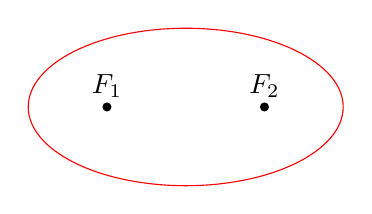
\begin{tikzpicture}
		\tkzInit[xmin=-2,ymin=-1,xmax=2,ymax=1]
		\tkzGrid
		\tkzAxeXY
	
		\draw[red] ellipse (2 and 1);
		\filldraw (-1,0) circle (0.05)
			node[above]{$F_1$};
		\filldraw (1,0) circle (0.05)
			node[above]{$F_2$};
	\end{tikzpicture}
\end{center}
Un'ellissi ha due assi, uno maggiore uno minore. Loro semi-lunghezze (quindi i semi-assi) si 
denominano $a$ (che contiene i fuochi) e $b$.\\
I fuochi sono i due punti tali che preso un punto $P\in\mathscr{E}$, 
$\overline{PF_1}+\overline{PF_2} = 2a$.
\begin{equation*}
\mathscr{E}:\,\frac{x^2}{a^2}+\frac{y^2}{b^2}=1
\end{equation*}
Tra i semi-assi vige la seguente propriet�
\begin{equation*}
a^2-c^2=b^2
\end{equation*}
e quindi
\begin{equation*}
c = \begin{cases}
a^2-b^2,\, &\text{se } a > b\\
b^2-a^2,\, &\text{se } a < b
\end{cases}
\end{equation*}

\subsubsection{Eccentricit�}
L'eccentricit� � lo schiacciamento dell'ellisse sull'asse maggiore. � un valore compreso tra $0$ e 
$1$.\\
Se $a>b$
\begin{equation*}
e = \frac{c}{a} = \frac{\sqrt{a^2-b^2}}{a}=\sqrt{1-\frac{b^2}{a^2}}
\end{equation*}
Se $b>a$
\begin{equation*}
e = \frac{c}{b} = \sqrt{1-\frac{a^2}{b^2}}
\end{equation*}

\subsubsection{Area dell'ellisse}
\begin{equation*}
\mathscr{A}(\mathscr{E}) = ab\pi
\end{equation*}

\subsubsection{Tangenti all'ellisse}
Per trovare la tangente all'esllise abbiamo due modi:
\begin{equation*}
\frac{xx_0}{a^2}+\frac{yy_0}{b^2}=1
\end{equation*}
oppure fare il sistema tra la retta generica per $P$ e fare in modo che il discriminante si annulli:
\begin{align*}
\begin{dcases}
\frac{x^2}{a^2}+\frac{y^2}{b^2}=1\\
y-y_0=m(x-x_0)
\end{dcases}\rightarrow\\ \frac{\Delta}{4}=a^4m^2q^2-a^2(q^2-b^2)(b^2+a^2m^2) = 0
\end{align*}
Il vantaggio di questo secondo metodo � che pu� anche trovare le rette secanti ed esterne all'ellisse
(rispettivamente con $\dfrac{\Delta}{4}>0$ e $\dfrac{\Delta}{4}<0$). � sicuramente pi� laborioso e
difficile da ricordare.

\subsection{Iperbole}
\begin{center}
	\begin{tikzpicture}
		\tkzInit[xmin=-2,ymin=-2,xmax=2,ymax=2]
		\tkzGrid
		\tkzAxeXY
	
		\draw[domain=-2:2] plot ({0.5*cosh(\x)}, {0.5*sinh(\x)});
		\draw[domain=-2:2] plot ({-0.5*cosh(\x)}, {-0.5*sinh(\x)});
	\end{tikzpicture}
\end{center}

L'iperbole pu� essere descritta sia anlaliticamente sia in modo parametrico con le funzioni $\cosh$ e
$\sinh$.\\
I fuochi sono i due punti tali che per un punto $P\in\mathscr{I}$, 
$\lvert \overline{PF_1}-\overline{PF_1}\rvert=2a$.\\
L'equazione dell'iperbole con i fuochi su $x$ �
\begin{equation*}
\mathscr{I}:\,\frac{x^2}{a^2}-\frac{y^2}{b^2}=1
\end{equation*}
Quella con i fuochi su $y$ �
\begin{equation*}
\mathscr{I}:\,\frac{x^2}{a^2}-\frac{y^2}{b^2}=-1
\end{equation*}

Tra i parametri $a$ e $b$ vige che $a < c$ e $c^2 = a^2+b^2$.

\subsubsection{Asintoti}
Gli asintoti sono le rette che l'iperbole tende a raggiungere senza mai toccare
\begin{equation*}
y=\pm\frac{b}{a}x
\end{equation*}

	\subsubsection{Eccentricit�}
L'eccentricit� dell'iperbole � il rapporto
\begin{equation*}
e=\frac{c}{a}=\sqrt{1+\frac{b^2}{a^2}}
\end{equation*}
se l'iperbole ha i fuochi su $x$,
\begin{equation*}
e = \frac{c}{b}=\sqrt{1+\frac{a^2}{b^2}}
\end{equation*}
altrimenti. Si noti anche che $e > 1$ per ogni iperbole.

\subsubsection{Iperbole equilatera}
Se $a=b$, l'iperbole si definisce equilatera e le equazioni diventano 
\begin{equation*}
x^2-y^2=a^2
\end{equation*}
se $F\in x$,
\begin{equation*}
y^2-x^2=a^2
\end{equation*}
se $F\in y$.\\
Questo comporta che $c = a\sqrt{2}$ e che $e=\sqrt{2}$.\\\\
Pu� anche essere descritta l'iperbole in base agli asintoti e in tal caso diventa
\begin{equation*}
xy=k
\end{equation*}

\subsubsection{Formule di sdoppiamento}
Vengono ora riportate le formule di sdoppiamento che cambiano in base all'equazione dell'iperbole
\begin{center}
	\begin{tabular}{c|c}
		Equazione & Tangente\\\hline
		$\dfrac{x^2}{a^2}-\dfrac{y^2}{b^2}=1$ & $\dfrac{xx_0}{a^2}-\dfrac{yy_0}{b^2}=1$\\\hline
		$\dfrac{x^2}{a^2}-\dfrac{y^2}{b^2}=-1$ & $\dfrac{xx_0}{a^2}-\dfrac{yy_0}{b^2}=-1$\\\hline
		$x^2-y^2=a^2$ & $xx_0-yy_0=a^2$\\\hline
		$x^2-y^2=-a^2$ & $xx_0-yy_0=-a^2$\\\hline
		$xy=k$ & $\dfrac{xy_0+x_0y}{2}-k=0$
	\end{tabular}
\end{center}

\subsubsection{Iperbole equilatera traslata}
Si trova molto spesso una versione traslata di un'iperbole. Questa � la sua generale forma
\begin{equation*}
y=\frac{ax+b}{cx+d}
\end{equation*}
E gli asintoti sono
\begin{equation*}
x=-\frac{d}{c}\qquad y=\frac{a}{c}
\end{equation*}
con il centro di simmetria
\begin{equation*}
O\left(-\frac{d}{c},\frac{a}{c}\right)
\end{equation*}